% Options for packages loaded elsewhere
\PassOptionsToPackage{unicode}{hyperref}
\PassOptionsToPackage{hyphens}{url}
%
\documentclass[
  11pt,
]{article}
\usepackage{amsmath,amssymb}
\usepackage{setspace}
\usepackage{iftex}
\ifPDFTeX
  \usepackage[T1]{fontenc}
  \usepackage[utf8]{inputenc}
  \usepackage{textcomp} % provide euro and other symbols
\else % if luatex or xetex
  \usepackage{unicode-math} % this also loads fontspec
  \defaultfontfeatures{Scale=MatchLowercase}
  \defaultfontfeatures[\rmfamily]{Ligatures=TeX,Scale=1}
\fi
\usepackage{lmodern}
\ifPDFTeX\else
  % xetex/luatex font selection
\fi
% Use upquote if available, for straight quotes in verbatim environments
\IfFileExists{upquote.sty}{\usepackage{upquote}}{}
\IfFileExists{microtype.sty}{% use microtype if available
  \usepackage[]{microtype}
  \UseMicrotypeSet[protrusion]{basicmath} % disable protrusion for tt fonts
}{}
\makeatletter
\@ifundefined{KOMAClassName}{% if non-KOMA class
  \IfFileExists{parskip.sty}{%
    \usepackage{parskip}
  }{% else
    \setlength{\parindent}{0pt}
    \setlength{\parskip}{6pt plus 2pt minus 1pt}}
}{% if KOMA class
  \KOMAoptions{parskip=half}}
\makeatother
\usepackage{xcolor}
\usepackage[margin=2.5cm]{geometry}
\usepackage{longtable,booktabs,array}
\usepackage{calc} % for calculating minipage widths
% Correct order of tables after \paragraph or \subparagraph
\usepackage{etoolbox}
\makeatletter
\patchcmd\longtable{\par}{\if@noskipsec\mbox{}\fi\par}{}{}
\makeatother
% Allow footnotes in longtable head/foot
\IfFileExists{footnotehyper.sty}{\usepackage{footnotehyper}}{\usepackage{footnote}}
\makesavenoteenv{longtable}
\usepackage{graphicx}
\makeatletter
\newsavebox\pandoc@box
\newcommand*\pandocbounded[1]{% scales image to fit in text height/width
  \sbox\pandoc@box{#1}%
  \Gscale@div\@tempa{\textheight}{\dimexpr\ht\pandoc@box+\dp\pandoc@box\relax}%
  \Gscale@div\@tempb{\linewidth}{\wd\pandoc@box}%
  \ifdim\@tempb\p@<\@tempa\p@\let\@tempa\@tempb\fi% select the smaller of both
  \ifdim\@tempa\p@<\p@\scalebox{\@tempa}{\usebox\pandoc@box}%
  \else\usebox{\pandoc@box}%
  \fi%
}
% Set default figure placement to htbp
\def\fps@figure{htbp}
\makeatother
\setlength{\emergencystretch}{3em} % prevent overfull lines
\providecommand{\tightlist}{%
  \setlength{\itemsep}{0pt}\setlength{\parskip}{0pt}}
\setcounter{secnumdepth}{5}
\usepackage{fvextra}
\usepackage{setspace}
\onehalfspacing
\DefineVerbatimEnvironment{Highlighting}{Verbatim}{breaklines,commandchars=\\\{\}}
\DefineVerbatimEnvironment{verbatim}{Verbatim}{breaklines,fontsize=\small}
\RecustomVerbatimEnvironment{verbatim}{Verbatim}{breaklines,fontsize=\small}
\usepackage{bookmark}
\IfFileExists{xurl.sty}{\usepackage{xurl}}{} % add URL line breaks if available
\urlstyle{same}
\hypersetup{
  pdftitle={Crop protocols},
  pdfauthor={Peñaloza-Bojacá, G.F.; Villarreal Lab.},
  hidelinks,
  pdfcreator={LaTeX via pandoc}}

\title{Crop protocols}
\author{Peñaloza-Bojacá, G.F.; Villarreal Lab.}
\date{2025-09}

\begin{document}
\maketitle

{
\setcounter{tocdepth}{3}
\tableofcontents
}
\setstretch{1.5}
\section{Introduction}\label{introduction}

Protocols for the preparation and use of different culture media applied
to for \emph{Hornworts, Cyanobacteria, Cycas and Zamia Seedlings}. Each
section includes media composition, step-by-step preparation, and notes
for practical application used in the Villarreal Lab.

\section{Hatcher medium (AG) for Hornwort solid and liquid
culture}\label{hatcher-medium-ag-for-hornwort-solid-and-liquid-culture}

Optimized using Anthoceros agrestis OXFORD, Fay-Wei Li (Andika Gunadi
(last updated 7/26/2021))

See \emph{Hatcher, Raymond E.Towards the Establishment of a Pure Culture
Collection of Hepaticae, 1965. DOI: 10.2307/3241021}

\subsection{Stock solutions}\label{stock-solutions}

\textbf{NOTE:} Gary Horvath can make Hatcher Nutrient Stocks A, B, and
Iron stock. Van Eck lab makes 10mg/ml Hygromycin stock -- ask before
using. Please make your own filter-sterilized MES buffer (pH 6.5), any
filter-sterilized antibiotic stock, and any other stock solution for
modification of your Hatcher medium.

\begin{figure}

{\centering 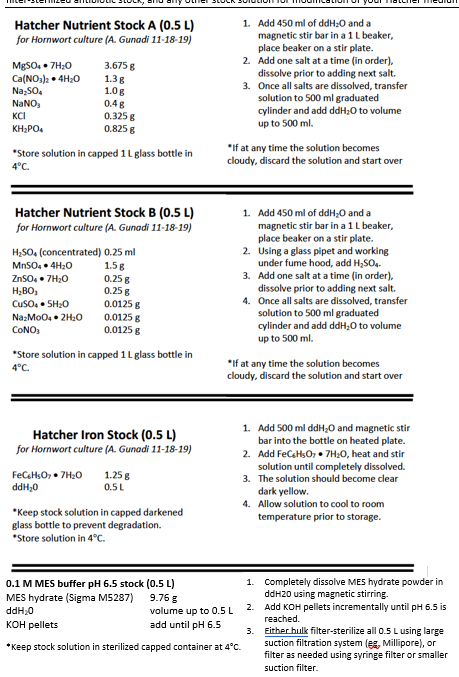
\includegraphics[width=0.6\linewidth]{Figuras/Stock} 

}

\caption{Hatcher Nutrient Stocks}\label{fig:unnamed-chunk-1}
\end{figure}

\begin{itemize}
\tightlist
\item
  In our laboratory we have MES (sigma 1317 liquid at 1M)
\item
  To dissolve \textbf{FeC₆H₅O₇ (ferric ammonium citrate)} more easily,
  it is recommended to place the solution on a magnetic stirrer and
  gently heat while stirring.
\end{itemize}

\subsection{To make 1 Liter medium}\label{to-make-1-liter-medium}

\begin{longtable}[]{@{}ll@{}}
\caption{\textbf{Composition of AG Medium (per 1 L)}}\tabularnewline
\toprule\noalign{}
Component & Amount \\
\midrule\noalign{}
\endfirsthead
\toprule\noalign{}
Component & Amount \\
\midrule\noalign{}
\endhead
\bottomrule\noalign{}
\endlastfoot
Hatcher Stock A & 100 ml \\
Hatcher Stock B & 3 ml \\
Hatcher Iron Stock & 1 ml \\
Ammonium nitrate & 0.4 g (0.4 g/L final) \\
Sucrose (optional for faster growth) & 2 g (0.2\% final) \\
Gelzan (solid medium) & 4 g \\
MES buffer (0.1 M MES, pH 6.5) & 50 ml \\
ddH2O & up to 950 ml \\
\end{longtable}

\begin{longtable}[]{@{}ll@{}}
\caption{\textbf{Optional Additives and Selection Agents for AG
Medium}}\tabularnewline
\toprule\noalign{}
Component & Amount \\
\midrule\noalign{}
\endfirsthead
\toprule\noalign{}
Component & Amount \\
\midrule\noalign{}
\endhead
\bottomrule\noalign{}
\endlastfoot
Activated Charcoal (Sigma C-3345) & 100 mg (100 mg/L final) \\
1 mg/ml filtered BA stock & 2.25 ml (10 nM final) \\
300 mg/ml filtered Timentin & 1 ml (300 mg/L final) \\
10 mg/ml filtered Hygromycin & 1 ml (10 mg/L final) \\
1 mM 2-Fluoroadenine (in DMSO) & 5 ml (5 µM final) \\
Benomyl (in DMSO) & 2.5 mg/L final \\
Imazalil (in water) & 20 µg/L final \\
Miconazole (in DMSO) & 10 mg/L final \\
Clomitrazole (in DMSO) & 10 µg/L final \\
Erythromycin (in DMSO) & 100 mg/L final \\
\end{longtable}

Store sterilized media in an autoclave at 4°C for up to 4 months. For
solid media, keep Petri dishes with the media facing down to prevent
liquefaction.

\textbf{Selection agents:} Hygromycin: Selects for plant tissues
expressing HygR gene (hptII) 2-Fluoroadenine: Selects for plant tissues
with knocked-out or -down endogenous APT gene

\textbf{Antimicrobials:} Against general bacterial contamination:
Timentin Against general fungal contamination: Benomyl, Imazalil,
Miconazole, Clomitrazole Against cyanobacteria: Erythromycin

In our laboratory, for bacterial control, a mixture of \emph{Penicillin
G} (100 ml k U/L), \emph{Tetracycline} (10 mg/L), and
\emph{Streptomycin} (72 k U/L) can be used in each 1 L of media.

For fungal control, \emph{Ketaconazole} (5 mg/L) or \emph{Cycloexamide}
(50 mg/L) diluted in MDSO can be used in each 1 L of media.

\subsection{Protocol for AG}\label{protocol-for-ag}

\begin{enumerate}
\def\labelenumi{\arabic{enumi}.}
\tightlist
\item
  In a beaker, add \textasciitilde500 ml ddH2O first, then mix
  components (Stock A+ stock B + Ammonium nitrate + Sucrose + Iron Stock
  ) in solution using magnetic stirrer.
\item
  Add ddH2O to 950 ml total.
\item
  While stirring, add KOH using dropper to reach pH 6.5.
\item
  Divide the Gelzan into two 1 Liter bottles (for solid medium only).
\item
  Add 425 ml of the liquid solution into each bottle, no need to mix.
\item
  Loosely cap the bottles, then autoclave for 20 min in liquid setting.
\item
  After autoclaving, cool media in water bath, mix occasionally until
  \textasciitilde55°C.
\item
  Add filtered \textbf{MES buffer} (pH 6.5) to 5 mM and BA stock to 10
  nM final concentrations, mix well.
\item
  Add any other selection agent (s) and antimicrobials as needed. Mix
  well. For solid media, pour into tall petri dishes at
  \textasciitilde35ml per dish. For liquid media, pour
  \textasciitilde50ml per sterile 100 ml flask.
\end{enumerate}

\section{KnopII medium (Nakazato et
al.~1999)}\label{knopii-medium-nakazato-et-al.-1999}

NAKAZATO T, KADOTA A \& WADA M. 1999. Photoinduction of Spore
Germination in Marchantia polymorpha L. is Mediated by Photosynthesis.
Plant Cell Physiol 40: 1014--1020.
\url{https://academic.oup.com/pcp/article-lookup/doi/10.1093/oxfordjournals.pcp.a029482}

Modified protocol for the culture of liverwort and hornwort (FEV/2025)
pH is adjusted to 5.5 with KOH before autoclaving. Sucrose and agar can
be added

\begin{longtable}[]{@{}ll@{}}
\caption{\textbf{Composition of Knop II Medium (per 1
L)}}\tabularnewline
\toprule\noalign{}
Component & Amount \\
\midrule\noalign{}
\endfirsthead
\toprule\noalign{}
Component & Amount \\
\midrule\noalign{}
\endhead
\bottomrule\noalign{}
\endlastfoot
KNO₃ & 125 mg \\
Ca(NO₃)₂·4H₂O & 500 mg \\
MgSO₄·7H₂O & 125 mg \\
KH₂PO₄ & 125 mg \\
FeCl₃·6H₂O & 10 mg \\
Sucrose (optional) & 3 g (0.3\%) \\
Agar (solid medium) & 3 g (0.3\%) \\
\end{longtable}

\textbf{Agar used at 0.5\% (Bacto-agar) or 0.3\% (Gelzan agar)}

\subsection{Stock solutions}\label{stock-solutions-1}

\begin{longtable}[]{@{}ll@{}}
\caption{\textbf{Knop II Medium Stocks (Dissolve the reagents in 50 ml
of deionized water)}}\tabularnewline
\toprule\noalign{}
Component & Amount \\
\midrule\noalign{}
\endfirsthead
\toprule\noalign{}
Component & Amount \\
\midrule\noalign{}
\endhead
\bottomrule\noalign{}
\endlastfoot
KNO₃ & 3.125 g \\
Ca(NO₃)₂·4H₂O & 12.5 g \\
MgSO₄·7H₂O & 3.125 g \\
KH₂PO₄ & 3.125 g \\
FeCl₃·6H₂O & 0.5 g \\
\end{longtable}

Add 2 ml of each stock to 1 L of distilled (ddH2O) water

\begin{longtable}[]{@{}ll@{}}
\caption{\textbf{Optional Additives and Selection Agents for KnopII
Medium}}\tabularnewline
\toprule\noalign{}
Component & Amount \\
\midrule\noalign{}
\endfirsthead
\toprule\noalign{}
Component & Amount \\
\midrule\noalign{}
\endhead
\bottomrule\noalign{}
\endlastfoot
300 mg/ml filtered Timentin & 1 ml (300 mg/L final) \\
10 mg/ml filtered Hygromycin & 1 ml (10 mg/L final) \\
1 mM 2-Fluoroadenine (in DMSO) & 5 ml (5 µM final) \\
Benomyl (in DMSO) & 2.5 mg/L final \\
Imazalil (in water) & 20 µg/L final \\
Miconazole (in DMSO) & 10 mg/L final \\
Clomitrazole (in DMSO) & 10 µg/L final \\
Erythromycin (in DMSO) & 100 mg/L final \\
\end{longtable}

Store sterilized media in an autoclave at 4°C for up to 4 months. For
solid media, keep Petri dishes with the media facing down to prevent
liquefaction.

\textbf{Selection agents:} - Hygromycin: Selects for plant tissues
expressing HygR gene (hptII) - 2-Fluoroadenine: Selects for plant
tissues with knocked-out or -down endogenous APT gene

\textbf{Antimicrobials:} - Against general bacterial contamination:
Timentin - Against general fungal contamination: Benomyl, Imazalil,
Miconazole, Clomitrazole - Against cyanobacteria: Erythromycin

In our laboratory, for bacterial control, a mixture of: -
\emph{Penicillin G} (100 ml k U/L); - \emph{Tetracycline} (10 mg/L); -
\emph{Streptomycin} (72 k U/L) can be used in each 1 L of media.

For fungal control, \emph{Ketaconazole} (5 mg/L) or \emph{Cycloexamide}
(50 mg/L) diluted in MDSO can be used in each 1 L of media.

\begin{itemize}
\tightlist
\item
  To dissolve \textbf{FeCl₃·6H₂O} more easily, it is recommended to
  place the solution on a magnetic stirrer and gently heat while
  stirring.
\end{itemize}

\subsection{Protocol for Knop II}\label{protocol-for-knop-ii}

\begin{enumerate}
\def\labelenumi{\arabic{enumi}.}
\tightlist
\item
  In a beaker, add \textasciitilde500 ml ddH2O first, then mix
  components in solution using magnetic stirrer.
\item
  Add ddH2O to 1000 ml total.
\item
  While stirring, add KOH using dropper to reach pH 5.5.
\item
  Divide the agar (example Gelzan agar) into two 1 Liter bottles (for
  solid medium only).
\item
  Add 500 ml of the liquid solution into each bottle, no need to mix.
\item
  Loosely cap the bottles, then autoclave for 20 min in liquid setting.
\item
  After autoclaving, cool media in water bath, mix occasionally until
  \textasciitilde55°C.
\item
  Add antimicrobials as needed (After autoclaving). Mix well. For solid
  media, pour into tall petri dishes at \textasciitilde35ml per dish.
\end{enumerate}

\section{Cyanobacteria -- BG-11
Medium}\label{cyanobacteria-bg-11-medium}

BG-11 medium (Rippka 1979) is one of the most widely used media for
culturing cyanobacteria.\\
It can be prepared as a concentrated stock and diluted for immediate
use.

\subsection{Stock Solutions}\label{stock-solutions-2}

\begin{longtable}[]{@{}ll@{}}
\caption{Standard BG-11 Stock Solutions (quantities per 200 ml
ddH₂O)}\tabularnewline
\toprule\noalign{}
Product & Amount\_in\_200ml \\
\midrule\noalign{}
\endfirsthead
\toprule\noalign{}
Product & Amount\_in\_200ml \\
\midrule\noalign{}
\endhead
\bottomrule\noalign{}
\endlastfoot
Solution 1: Disodium EDTA (Na2C10H14O8N2·2H2O) & 0.2 g \\
Solution 2: Citric acid (C6H8O7·H2O) & 1.2 g \\
Solution 3: Sodium nitrate (NaNO3) & 30 g \\
Solution 4: Dipotassium phosphate (K2HPO4) & 6.12 g \\
Solution 5: Magnesium sulfate (MgSO4·7H2O) & 15 g \\
Solution 6: Calcium chloride dihydrate (CaCl2·2H2O) & 7.2 g \\
Solution 7: Sodium carbonate anhydrous (Na2CO3) & 4 g \\
Solution 8: Ferric ammonium citrate (Fe 16.5--18.5\%) & 1.2 g \\
\end{longtable}

\emph{Solution 9: Micronutrients}

\begin{longtable}[]{@{}ll@{}}
\caption{Micronutrients for BG-11 Stock (per 200 ml
ddH₂O)}\tabularnewline
\toprule\noalign{}
Component & Amount\_in\_200ml \\
\midrule\noalign{}
\endfirsthead
\toprule\noalign{}
Component & Amount\_in\_200ml \\
\midrule\noalign{}
\endhead
\bottomrule\noalign{}
\endlastfoot
Boric acid (H3BO3) & 0.572 g \\
Manganese chloride (MnCl2·4H2O) & 0.36 g \\
Zinc sulfate (ZnSO4·7H2O) & 0.044 g \\
Copper sulfate (CuSO4·5H2O or 4\% w/v solution) & 0.016 g or 0.4 ml \\
Sodium molybdate (Na2MoO4·2H2O) & 0.078 g \\
Cobalt chloride (CoCl2·6H2O) & 0.008 g \\
\end{longtable}

\subsection{Protocol for Standard BG-11
Medium}\label{protocol-for-standard-bg-11-medium}

To prepare \textbf{1 L of culture medium}:

\begin{enumerate}
\def\labelenumi{\arabic{enumi}.}
\tightlist
\item
  Add \textbf{1 ml} of each stock solution listed above (except
  solutions 4, 8 and 9) into \textbf{991 ml} of deionized water.
\item
  pH should be adjusted to 7.44 - 7.48.
\item
  Addition the Gelzan agar (for solid medium only).
\item
  Sterilize the medium by autoclaving (20 min in liquid setting)
\item
  After autoclaving, cool media in water bath, mix occasionally until
  \textasciitilde55°C, and add \textbf{1 ml} of each of the following
  stock solutions:

  \begin{itemize}
  \tightlist
  \item
    \textbf{Solution 4} (Dipotassium phosphate, K₂HPO₄)\\
  \item
    \textbf{Solution 8} (Ferric ammonium citrate, Fe 16.5--18.5\%)\\
  \item
    \textbf{Solution 9} (Micronutrients)\\
    These solutions must be \textbf{filter-sterilized (0.2 µm)}
    immediately before being added to the autoclaved medium.\\
  \end{itemize}
\item
  Add antimicrobials as needed (After autoclaving). Mix well. For solid
  media
\item
  pour into tall petri dishes at \textasciitilde35ml per dish.
\end{enumerate}

\textbf{Note:}

\begin{itemize}
\tightlist
\item
  To dissolve \textbf{ferric ammonium citrate (FeC₆H₅O₇)} more easily,
  it is recommended to place the solution on a magnetic stirrer and
  gently heat while stirring.
\item
  To prepare \textbf{nitrogen-free BG-11}, simply \textbf{omit stock
  solution 3 (NaNO₃)}.\\
\item
  For \textbf{solid media}, add \textbf{10 g/L of Bacto Agar™} to the
  preparation before autoclaving.
\item
  Store Petri dishes with \textbf{solid medium lid-side up} to avoid
  liquefaction or structural damage to the medium.
\item
  Store sterilized media in fridge at 4°C for up to 5 months.
\end{itemize}

\emph{Antimicrobials:}

\begin{itemize}
\tightlist
\item
  Against general bacterial contamination: Timentin
\item
  Against general fungal contamination: Benomyl, Imazalil, Miconazole,
  Clomitrazole
\item
  Against cyanobacteria: Erythromycin
\end{itemize}

In our laboratory, for bacterial control, a mixture of:

\begin{itemize}
\tightlist
\item
  \emph{Penicillin G} (100 ml k U/L);
\item
  \emph{Tetracycline} (10 mg/L);
\item
  \emph{Streptomycin} (72 k U/L) can be used in each 1 L of media.
\end{itemize}

\emph{fungal control}

\begin{itemize}
\tightlist
\item
  \emph{Ketaconazole} (5 mg/L) \textbf{or} \emph{Cycloexamide} (50 mg/L)
  diluted in MDSO can be used in each 1 L of media.
\end{itemize}

\subsection{Final Mineral Concentrations in BG-11
Medium}\label{final-mineral-concentrations-in-bg-11-medium}

\begin{longtable}[]{@{}lr@{}}
\caption{Final Mineral Concentrations in BG-11 Medium
(mg/L)}\tabularnewline
\toprule\noalign{}
Mineral & Concentration\_mgL \\
\midrule\noalign{}
\endfirsthead
\toprule\noalign{}
Mineral & Concentration\_mgL \\
\midrule\noalign{}
\endhead
\bottomrule\noalign{}
\endlastfoot
Disodium EDTA (Na2C10H14O8N2·2H2O) & 1.00 \\
Citric acid (C6H8O7·H2O) & 6.00 \\
Sodium nitrate (NaNO3) & 150.00 \\
Dipotassium phosphate (K2HPO4) & 30.60 \\
Magnesium sulfate (MgSO4·7H2O) & 75.00 \\
Calcium chloride dihydrate (CaCl2·2H2O) & 36.00 \\
Sodium carbonate anhydrous (Na2CO3) & 20.00 \\
Ferric ammonium citrate (Fe 16.5--18.5\%) & 6.00 \\
Boric acid (H3BO3) & 2.86 \\
Manganese chloride (MnCl2·4H2O) & 1.81 \\
Zinc sulfate (ZnSO4·7H2O) & 0.22 \\
Copper sulfate (CuSO4·5H2O) & 0.08 \\
Sodium molybdate (Na2MoO4·2H2O) & 0.39 \\
Cobalt chloride (CoCl2·6H2O) & 0.04 \\
\end{longtable}

\section{20:20:20 Fertilizer}\label{fertilizer}

The balanced NPK fertilizer \textbf{20:20:20} is commonly used for
cultivating \emph{Zamia} seedlings in growth chambers and greenhouse
conditions.\\
It provides macronutrients (N, P, K) and essential micronutrients in
chelated form.

\begin{longtable}[]{@{}ll@{}}
\caption{Composition of 20--20--20 Fertilizer}\tabularnewline
\toprule\noalign{}
Component & Content \\
\midrule\noalign{}
\endfirsthead
\toprule\noalign{}
Component & Content \\
\midrule\noalign{}
\endhead
\bottomrule\noalign{}
\endlastfoot
Total Nitrogen (N) & 20\% \\
Available Phosphoric Acid (P₂O₅) & 20\% \\
Soluble Potash (K₂O) & 20\% \\
Boron (B) & 0.02\% \\
Chelated Copper (Cu) & 0.05\% \\
Chelated Iron (Fe) & 0.10\% \\
Chelated Manganese (Mn) & 0.05\% \\
Molybdenum (Mo) & 0.0005\% \\
Chelated Zinc (Zn) & 0.05\% \\
EDTA (chelating agent) & 1.2\% \\
\end{longtable}

\subsection{Protocol}\label{protocol}

\begin{itemize}
\tightlist
\item
  Prepare a \textbf{solution} by dissolving \textbf{200 mg of 20--20--20
  fertilizer} in \textbf{1 L of deionized steril water}.

  \begin{itemize}
  \tightlist
  \item
    This yields a solution with approximately \textbf{10 mg of N per 50
    ml}.\\
  \end{itemize}
\item
  Apply to plants as follows:

  \begin{itemize}
  \tightlist
  \item
    \textbf{Greenhouse:} water each plant with 25 ml, \textbf{twice per
    week}.\\
  \item
    \textbf{Growth chamber:} water each plant with 50 ml, \textbf{once
    per week}.\\
  \end{itemize}
\item
  After some weeks of growth, switch fertilization to BG-11 medium for
  further cultivation.
\end{itemize}

\textbf{Note:} Fertilizer solution should be prepared fresh and
sterilized after addition to avoid microbial contamination.

\subsection{Laboratory Note -- Growth Chamber Fertilizer Use for
Stéphanie (Nov 2,
2021)}\label{laboratory-note-growth-chamber-fertilizer-use-for-stuxe9phanie-nov-2-2021}

This note comes from laboratory files and is included here for
reference.

\subsubsection{Tasks}\label{tasks}

\begin{enumerate}
\def\labelenumi{\arabic{enumi}.}
\tightlist
\item
  Water plants 1--2 times per week, prepare the fertilizer (sterilize
  after adding 1 g of fertilizer {[}20:20:20{]}), see below.\\
\item
  Measure the quantity of leaves and leaflets, and take photos of the
  plants in the greenhouse (once every 2--3 weeks).\\
\item
  In 3--4 weeks, begin using BG-11 medium (see Zamia article in
  \emph{Symbiosis}) with seedlings in the growth chamber only.\\
  The solutions are already prepared; they just need to be mixed. A
  graduate student will assist you.\\
\item
  In 4 weeks, germinate new \emph{Zamia} seeds (a different species) in
  sterile vermiculite/sand. A graduate student will assist you.\\
\item
  In 6 weeks, transfer the seedlings, check morphology, presence of
  coralloid roots, and preserve cyanobacteria for metagenomic analyses.
  A graduate student will assist you.
\end{enumerate}

\subsubsection{Student Message}\label{student-message}

The important content is in the folder \textbf{``photo leaf area''},
where weekly photos of leaf area were taken.\\
Leaf surface can be measured using ImageJ.\\
There is also an Excel file \textbf{``Feuille de données serre''} with
height and leaf counts.\\
For methods, refer to the research proposal. For fertilization details,
see the document \textbf{``Arrosage des plantes''}.

\subsubsection{Important Files in the
Folder}\label{important-files-in-the-folder}

\begin{itemize}
\tightlist
\item
  Informations serre\\
\item
  Template feuille de données\\
\item
  Feuille de données -- serres\\
\item
  Photo leaf area\\
\item
  Culture BG-11 cyanobacteries
\end{itemize}

\subsubsection{Watering Schedule}\label{watering-schedule}

\begin{itemize}
\tightlist
\item
  \textbf{Greenhouse:} 25 ml/plant, twice per week.\\
\item
  \textbf{Growth chamber:} 50 ml/plant, once per week with fertilizer
  (switch later to BG-11).
\end{itemize}

\begin{figure}

{\centering 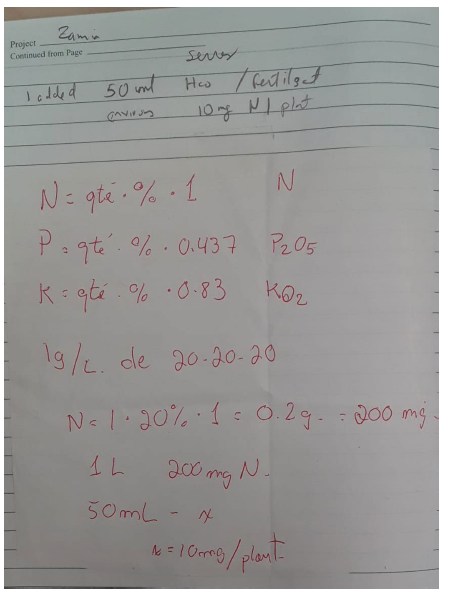
\includegraphics[width=0.7\linewidth]{Figuras/202020} 

}

\caption{Laboratory note on fertilizer 20-20-20}\label{fig:fert2020_img}
\end{figure}

\subsection{\texorpdfstring{Laboratory Note -- Watering of \emph{Zamia
furfuracea} (June 21,
2021)}{Laboratory Note -- Watering of Zamia furfuracea (June 21, 2021)}}\label{laboratory-note-watering-of-zamia-furfuracea-june-21-2021}

This note is preserved from internal lab instructions. It is \textbf{not
part of the standardized protocol}, but documents how watering and
fertilization were carried out in the greenhouse.

\subsubsection{\texorpdfstring{Arrosage des plants de \emph{Zamia
furfuracea}}{Arrosage des plants de Zamia furfuracea}}\label{arrosage-des-plants-de-zamia-furfuracea}

\begin{itemize}
\tightlist
\item
  Fill \textbf{10 bottles} with tap water (not distilled water) up to
  900 ml.\\
  \emph{Bottles are stored in lab 2211 next to the hood.}\\
\item
  Autoclave the bottles (liquid cycle, 20 minutes).

  \begin{itemize}
  \tightlist
  \item
    Preferably autoclave in the morning or the day before to allow more
    cooling time.\\
  \item
    It is also recommended to use the autoclave in the basement, since
    the sterilization service slows down during summer.\\
  \end{itemize}
\item
  Water the plants.
\end{itemize}

\subsubsection{Fertilizer addition (Monday, June
21)}\label{fertilizer-addition-monday-june-21}

\begin{itemize}
\tightlist
\item
  Fertilizer used: \textbf{20--20--20} (see storage location below).\\
\item
  Add \textbf{0.5 g fertilizer per bottle} using the balance.

  \begin{itemize}
  \tightlist
  \item
    It is advisable to bring a small spoon from the lab to measure the
    fertilizer.
  \end{itemize}
\end{itemize}

\subsubsection{Important information}\label{important-information}

\begin{itemize}
\tightlist
\item
  Plants must be watered \textbf{on Mondays and Thursdays}.\\
\item
  The greenhouse doors are locked:

  \begin{itemize}
  \tightlist
  \item
    The \textbf{first door} requires a code: \texttt{225323}Check with
    Juan Carlos Villarreal.
  \end{itemize}
\end{itemize}

\begin{figure}

{\centering 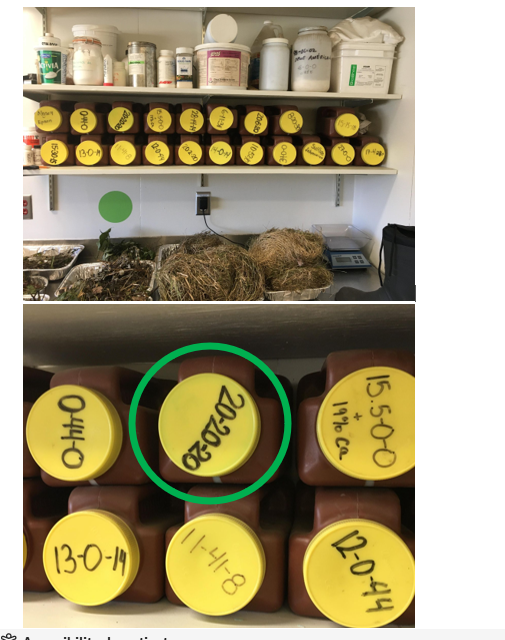
\includegraphics[width=0.48\linewidth]{Figuras/fertilizanteA} 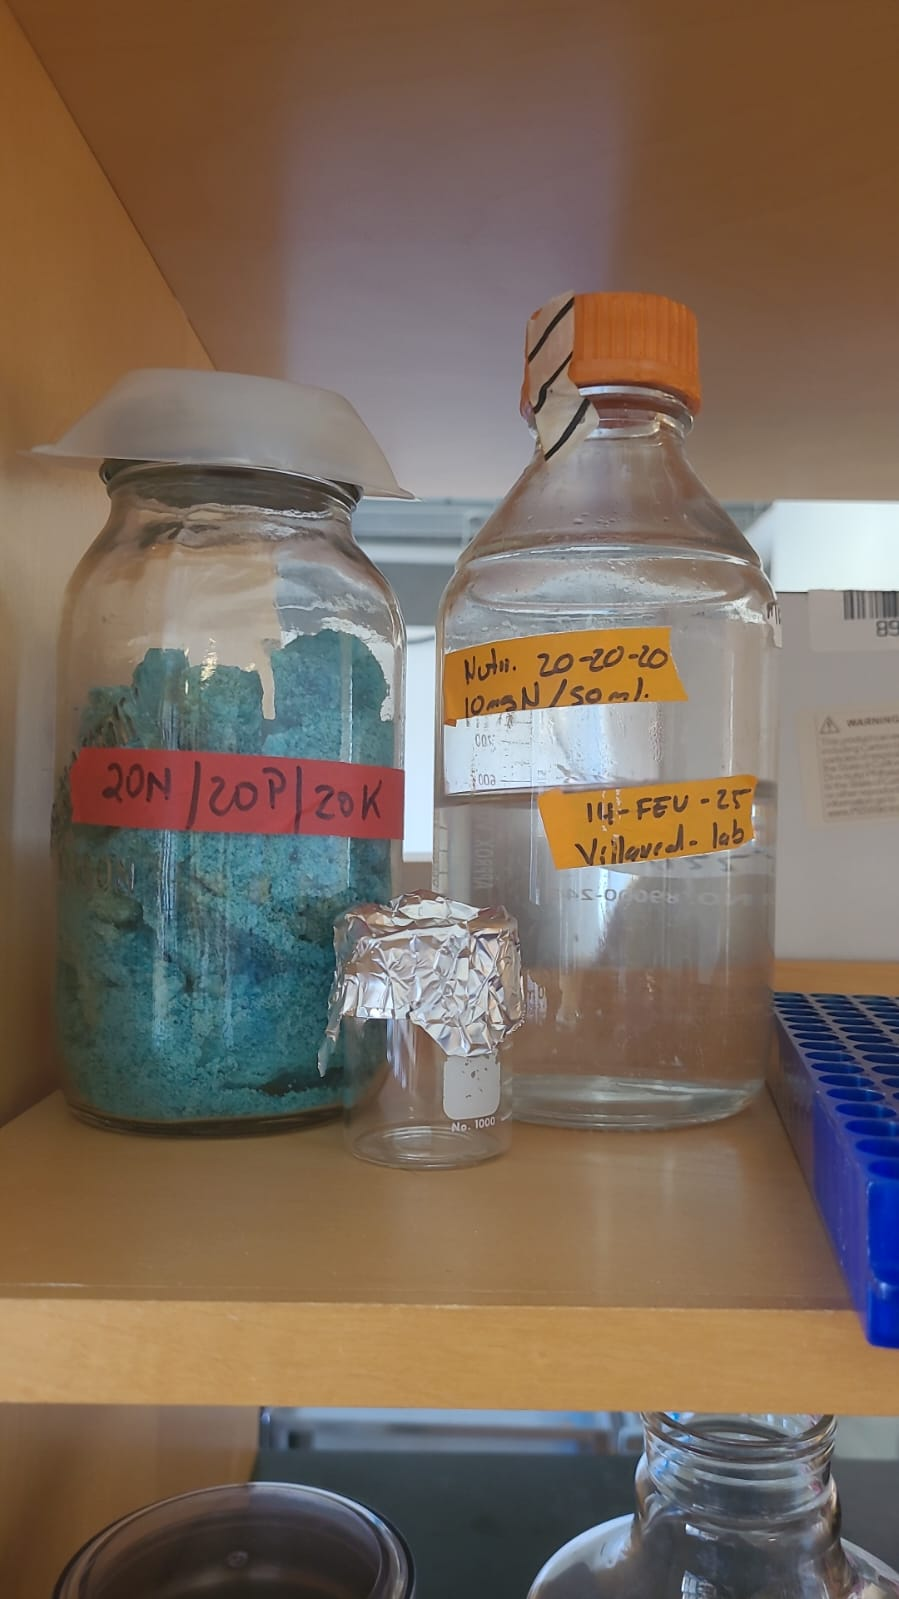
\includegraphics[width=0.48\linewidth]{Figuras/fertilizante} 

}

\caption{Laboratory Note – Fertilizer preparation. A: Sala Forestal. B: Stock 20-20-20 (Lab 2211).}\label{fig:fert2020_imgs}
\end{figure}

\section{Seed Sterilization -- Zamia and
Cycas}\label{seed-sterilization-zamia-and-cycas}

\begin{itemize}
\item
  Remove the seed coat (testa) carefully with a scalpel or razor blade.

  \begin{itemize}
  \tightlist
  \item
    Avoid using a very sharp or thin blade that could damage the
    endosperm or embryo.\\
  \item
    For seedlings, first wash vigorously with tap water to remove all
    soil.
  \end{itemize}
\item
  Expose the seeds to UV light for \textbf{30 minutes} to reduce
  contamination.
\item
  Prepare the disinfection solutions:

  \begin{itemize}
  \tightlist
  \item
    \textbf{Fungicide solution:} 300 ml deionized water + 0.36 g
    fungicide.\\
  \item
    \textbf{Alcohol 97\%} (fresh).\\
  \item
    \textbf{Alcohol 70\%} (fresh).\\
  \item
    \textbf{Sterile distilled water} for rinsing.
  \end{itemize}
\item
  Sequential disinfection (one seed at a time using sterile forceps):

  \begin{itemize}
  \tightlist
  \item
    Dip in \textbf{97\% ethanol} for \textbf{30 seconds} (with gentle
    agitation).\\
  \item
    Transfer to \textbf{70\% ethanol} for \textbf{1 minute} (agitate
    gently).
  \item
    Transfer to sterile distilled water and rinse thoroughly.\\
  \item
    Transfer to \textbf{Fungicide solution} for \textbf{3 minute}
    (agitate gently).\\
  \item
    Place seeds on sterile paper towel to dry briefly.
  \end{itemize}
\item
  After drying, transfer seeds to prepared sterile containers with
  sterile perlite/vermiculite/sand or directly to culture medium,
  depending on experimental design.
\end{itemize}

\textbf{Laboratory Note} -- Additional Seed Cleaning Details

\begin{itemize}
\tightlist
\item
  Each seed was manipulated individually with large sterile forceps.\\
\item
  After the ethanol washes, seeds were transferred through a series of
  beakers containing alcohols and finally fungicide.\\
\item
  When all seeds had been processed, they were placed together in the
  fungicide solution and shaken vigorously for \textbf{3 minutes}.\\
\item
  Seeds were then dried on sterile paper towels before sowing.\\
\item
  For each container, 200 ml of deionized water was added after seed
  placement to maintain humidity.
\end{itemize}

\section{Coralloid Root Sterilization
Protocol}\label{coralloid-root-sterilization-protocol}

\emph{References} - Bell‐Doyon, P.; Laroche, J.; Saltonstall, K.;
Villarreal, J.C. Specialized Bacteriome Uncovered in the Coralloid Roots
of the Epiphytic Gymnosperm, \emph{Zamia pseudoparasitica}.
\emph{Environ. DNA} 2020, 1--11. \url{https://doi.org/10.1002/edn3.66}\\
- Sierra, A.M.; Toupin, S.; Alonso-García, M.; Villarreal, J.C.
Diversity of Symbiotic Cyanobacteria in Cycad Coralloid Roots Using a
Short-Read \emph{RbcL-X} Amplicon. \emph{Symbiosis} 2024, 92, 271--288.
\url{https://doi.org/10.1007/s13199-024-00972-w}

\subsection{Pre-processing Storage
Conditions}\label{pre-processing-storage-conditions}

\begin{itemize}
\tightlist
\item
  Coralloid roots should be stored on \textbf{ice in a hermetically
  sealed container at 4 °C} for no more than \textbf{2 hours} prior to
  laboratory processing.
\end{itemize}

\subsection{Required Materials}\label{required-materials}

\begin{itemize}
\tightlist
\item
  Double-distilled water (ddH₂O; autoclaved)\\
\item
  1\% Triton X-100 solution\\
\item
  1\% commercial bleach (sodium hypochlorite)\\
\item
  95\% ethanol\\
\item
  70\% ethanol\\
\item
  40\% ethanol\\
\item
  Sterile 1.5 ml microcentrifuge tubes (for DNA or RNA extraction)
\end{itemize}

\subsection{Surface Sterilization
Procedure}\label{surface-sterilization-procedure}

\begin{itemize}
\item
  \textbf{Initial Cleaning}: Rinse the coralloid roots thoroughly with
  autoclaved ddH₂O until all visible debris is removed.
\item
  \textbf{Detergent and Bleach Treatment}

  \begin{itemize}
  \tightlist
  \item
    Submerge the cleaned roots in \textbf{1\% Triton X-100} solution for
    \textbf{1 minute}.\\
  \item
    Immediately transfer them to \textbf{1\% commercial bleach} for an
    additional \textbf{1 minute}.
  \end{itemize}
\item
  \textbf{Rinse}: Rinse the roots thoroughly with \textbf{ddH₂O for 5
  minutes} to ensure complete removal of Triton X-100 and bleach
  residues.
\item
  \textbf{Ethanol Wash Series}

  \begin{itemize}
  \tightlist
  \item
    95\% ethanol for 30 seconds\\
  \item
    70\% ethanol for 60 seconds\\
  \item
    40\% ethanol for 120 seconds
  \end{itemize}
\item
  \textbf{Final Rinse}: Rinse the roots \textbf{three times with ddH₂O}
  to remove any residual ethanol.
\item
  \textbf{Storage}: Transfer the surface-sterilized coralloid roots into
  \textbf{sterile 1.5 ml microcentrifuge tubes} for subsequent DNA or
  RNA extraction.
\end{itemize}

\textbf{Notes} - It is recommended to complete the cleaning process and
immediately immerse the roots in \textbf{liquid nitrogen}.\\
- Frozen roots can be stored at \textbf{−80 °C}.\\
- For \textbf{RNA extractions}, keep roots in liquid nitrogen during
transport and throughout the initial stages of the extraction process.

\section{\texorpdfstring{Cultivation of \emph{Nostoc} in Liquid and
Solid
Media}{Cultivation of Nostoc in Liquid and Solid Media}}\label{cultivation-of-nostoc-in-liquid-and-solid-media}

\subsection{Medium}\label{medium}

\begin{itemize}
\tightlist
\item
  \textbf{BG-11 without nitrogen (BG-11₀)} -- prepared as stock
  following standard recipe, omitting NaNO₃.\\
\item
  \textbf{Cycloheximide} -- final concentration: \textbf{50 mg/L} (to
  inhibit eukaryotic contaminants).\\
\item
  \textbf{Optional for solid medium:} 10 g/L Bacto Agar™.
\end{itemize}

\subsection{Materials}\label{materials}

\begin{itemize}
\tightlist
\item
  BG-11₀ medium (liquid or solid base)\\
\item
  Cycloheximide (10 mg/ml sterile stock, filter sterilized)\\
\item
  Autoclaved Erlenmeyer flasks or sterile Petri dishes\\
\item
  Sterile pipettes and culture tools\\
\item
  Inoculum of \emph{Nostoc} (previously grown cultures)
\end{itemize}

\subsection{Protocol -- Liquid Medium}\label{protocol-liquid-medium}

\begin{itemize}
\tightlist
\item
  \textbf{Prepare the medium}

  \begin{itemize}
  \tightlist
  \item
    Autoclave BG-11₀ medium.\\
  \item
    Once cooled to room temperature, add cycloheximide to a final
    concentration of \textbf{50 mg/L}\\
  \end{itemize}
\item
  \textbf{Inoculation}

  \begin{itemize}
  \tightlist
  \item
    Transfer fresh \emph{Nostoc} filaments aseptically into sterile
    Erlenmeyer flasks containing BG-11₀ + cycloheximide.\\
  \item
    Typical working volume: \textbf{250 ml medium} in \textbf{500 ml
    flask}.\\
  \end{itemize}
\item
  \textbf{Incubation}

  \begin{itemize}
  \tightlist
  \item
    Grow cultures under continuous light or a 16/8 h light/dark cycle.\\
  \item
    Temperature: \textbf{25--28 °C}.\\
  \item
    Agitation: optional shaking at \textbf{100 -120 rpm} to prevent
    clumping and ensure aeration.
  \end{itemize}
\end{itemize}

\begin{figure}

{\centering 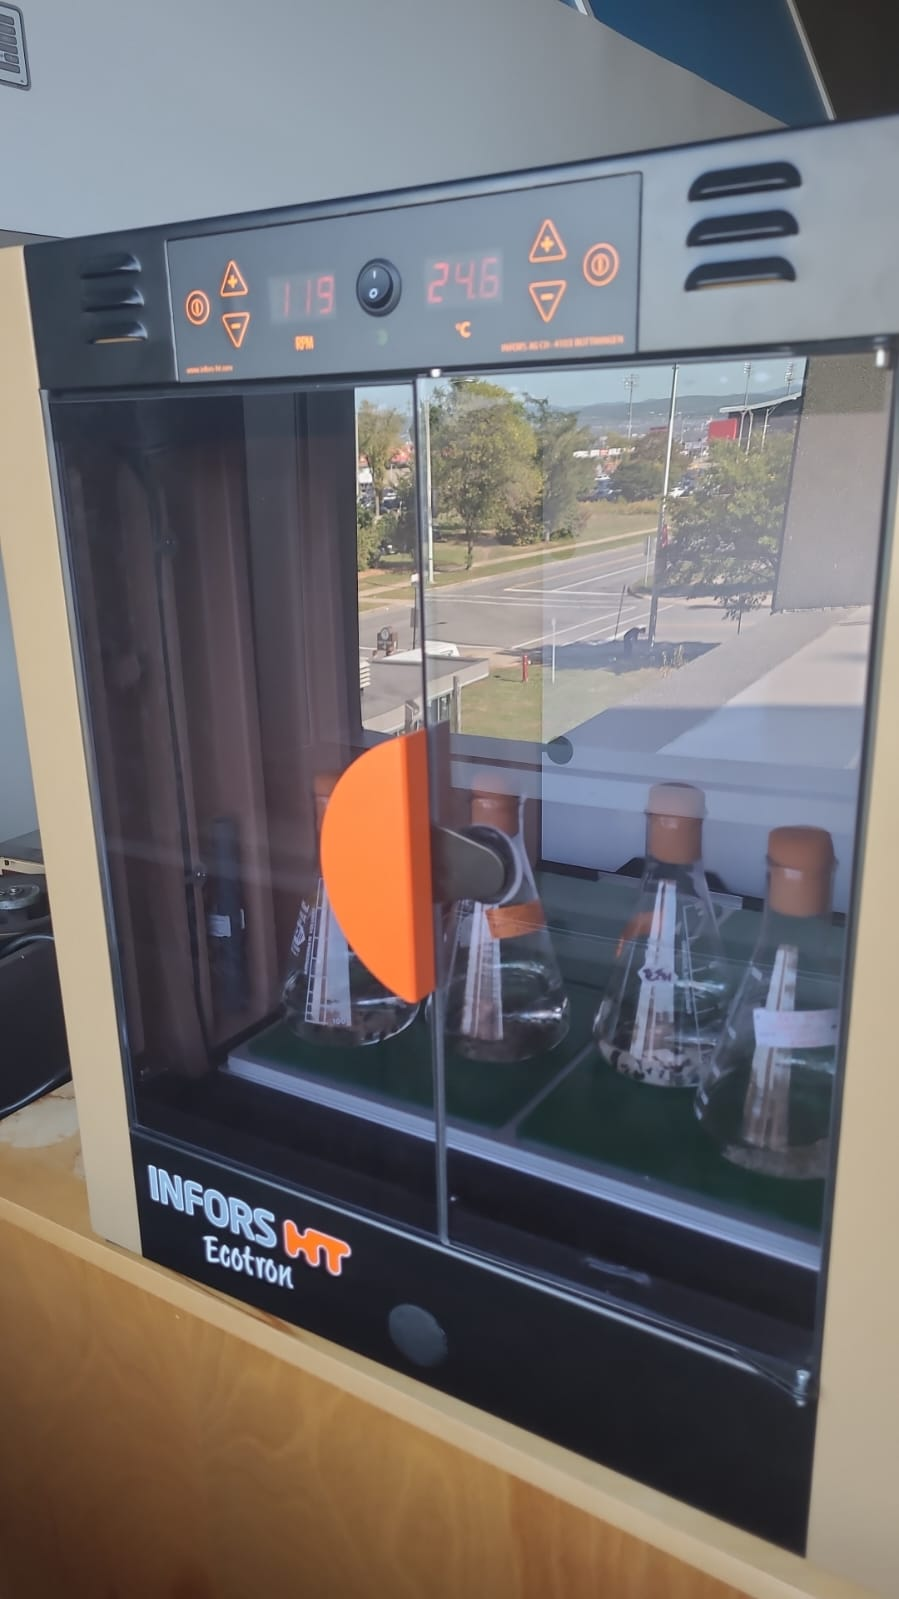
\includegraphics[width=0.32\linewidth]{Figuras/nostoc (1)} 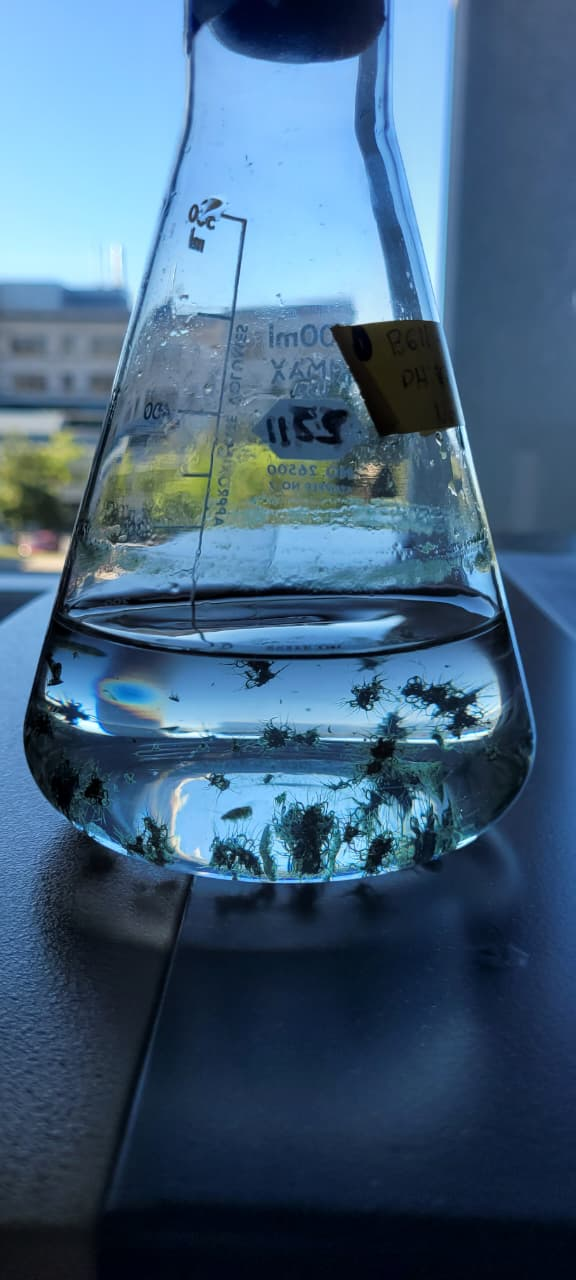
\includegraphics[width=0.32\linewidth]{Figuras/nostoc (2)} 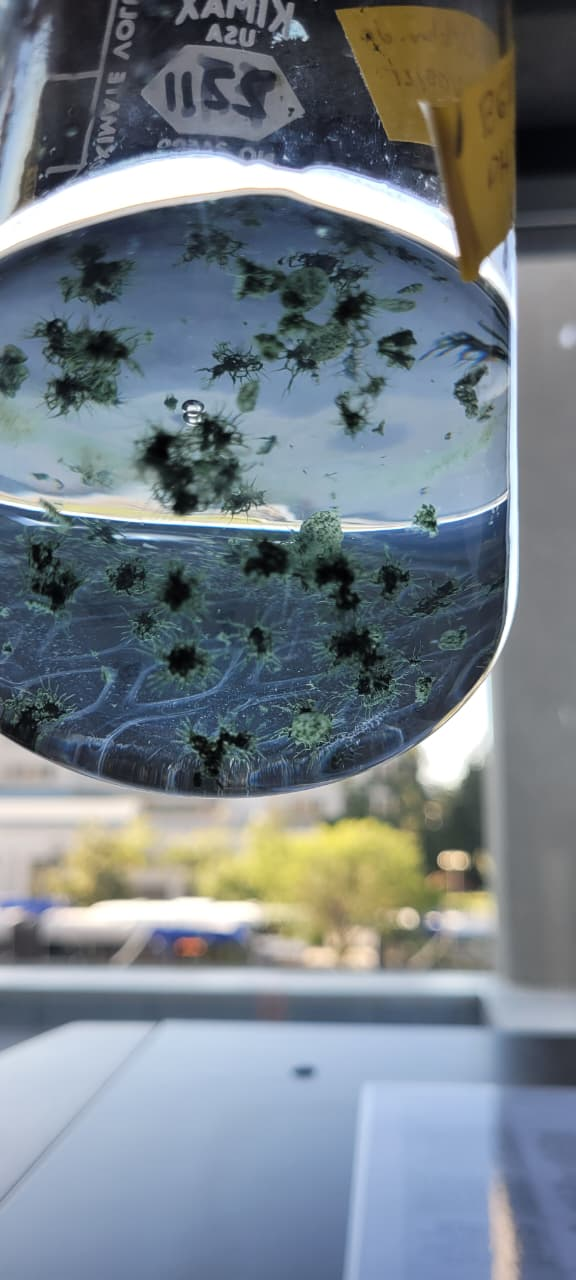
\includegraphics[width=0.32\linewidth]{Figuras/nostoc (3)} 

}

\caption{Nostoc cultivation on BG-11₀ medium.}\label{fig:nostoc_imgs}
\end{figure}

\subsection{Protocol -- Solid Medium}\label{protocol-solid-medium}

\begin{itemize}
\tightlist
\item
  \textbf{Prepare BG-11₀ agar plates}

  \begin{itemize}
  \tightlist
  \item
    Add \textbf{10 g/L Bacto Agar™} to BG-11₀ medium.\\
  \item
    Autoclave, cool to 55 °C, and add cycloheximide (50 mg/L final) by
    mixing thoroughly before pouring.\\
  \end{itemize}
\item
  \textbf{Inoculation}

  \begin{itemize}
  \tightlist
  \item
    Place small filaments or droplets of liquid inoculum onto the agar
    surface.\\
  \item
    Spread gently with sterile loop or glass rod.\\
  \end{itemize}
\item
  \textbf{Incubation}

  \begin{itemize}
  \tightlist
  \item
    Incubate plates at \textbf{25--28 °C}, under continuous light or
    16/8 h cycle.\\
  \item
    Maintain moderate humidity to prevent agar desiccation.\\
    \textbf{Notes}
  \end{itemize}
\item
  Cycloheximide is \textbf{fungistatic} and reduces eukaryotic
  contaminants but does not affect cyanobacteria like \emph{Nostoc}.\\
\item
  For long-term maintenance, transfer colonies or liquid cultures to
  fresh BG-11₀ medium every \textbf{3--4 weeks}.\\
\item
  Solid plates should be stored in sealed plastic bags or
  parafilm-wrapped to reduce drying.\\
\item
  Petri dishes containing solid medium should be \textbf{incubated in
  the inverted position} (agar side up, lid side down).\\
\item
  This prevents condensation from dripping onto the agar surface and
  reduces \textbf{evaporation} of the medium.
\end{itemize}

\end{document}
